% =============================================================================
\section{The chart-casting engine of Parashara's Light 7}
\label{sec:engine}
% =============================================================================

This section answers the central question: \emph{how does PL7 cast a chart?} Every
statement is graded \tagBIN, \tagNUM, \tagDOC\ or \tagINF\ as defined in
\autoref{sec:grades}. The software analysed is \texttt{PL7.exe}, a 32-bit Windows
executable linked on 1~August~2006 with the Microsoft Visual C++~6 linker against Qt~3.3.6
(\texttt{qt-mt336.dll}); its SHA-256 is \texttt{e530a346\ldots 35f9}.

\subsection{Ephemeris source and valid date range}
\label{sec:ephem}

PL7 does \emph{not} use the Swiss Ephemeris. It reads its own data files from
\texttt{Bin/}: \texttt{ephemdat.bin} (1.7~MB), \texttt{topos1.dat}, \texttt{topos2.dat},
\texttt{Topos3.dat} and \texttt{Topos.ndx} (planetary series), \texttt{approx.dat} and
\texttt{JUNCTION.DAT}. The start-up routine prints ``initialising ephemeris\ldots'' and
aborts with ``File missing: topos1.dat or topos2.dat'' if the series are absent; the
reader routine (\texttt{fcn.0055de40}) rejects dates outside the file's range with
``Invalid date for ephemeris'' and labels its internal frame \texttt{EQU2000}, i.e.\ the
series are stored as J2000 equatorial coordinates and rotated to the ecliptic of date
\tagBIN.

The transit cache (\autoref{sec:transit}) gives an external check of this range. Moon and
Rahu positions agree with the Swiss Ephemeris to better than one arcsecond for every
cached month from January~2020 to December~2048, and become wrong by up to
$\pm 5000''$ from 1~January~2049 onwards \tagNUM. The precise ephemeris therefore ends
with the year 2048; after that PL7 silently falls back to a coarse approximation
(the code references \texttt{approx.dat} with the messages ``error loading approx.dat''
and ``could not read approx.dat completely'') \tagINF. The lower bound is held in the
data file rather than in the executable and was not determined.

\begin{warnbox}\kpit A horary or muhurta chart in PL7 for a date in 2049 or later is computed
from the fallback approximation, and the program gives no warning. Kala Chakra's Swiss
Ephemeris files cover 1800--2399, so the two programs will disagree by arcminutes for
such dates, and PL7 is the one in error.\end{warnbox}

\subsection{Delta-T (the TT$-$UT correction)}
\label{sec:deltat}

PL7 ships \texttt{Bin/DELTAT.ASC}, a half-yearly table of $\Delta T$ from 1800.0
(12.578~s) to 1993.0 (59.122~s), dated March~1993 \tagBIN. For later dates it must
extrapolate. Fitting the Moon in the transit cache (the Moon moves $0.55''$ per second of
time, so a $\Delta T$ error shows up as a pure lunar offset) gives PL7's effective
$\Delta T$ as $83.0$~s in January~2020, rising linearly at $0.89$~s~yr$^{-1}$ to
$108.8$~s at the end of~2048 \tagNUM\ (\autoref{fig:deltat}). The true value has stayed
near $69$~s since 2020.

\begin{figure}[htbp]
  \centering
  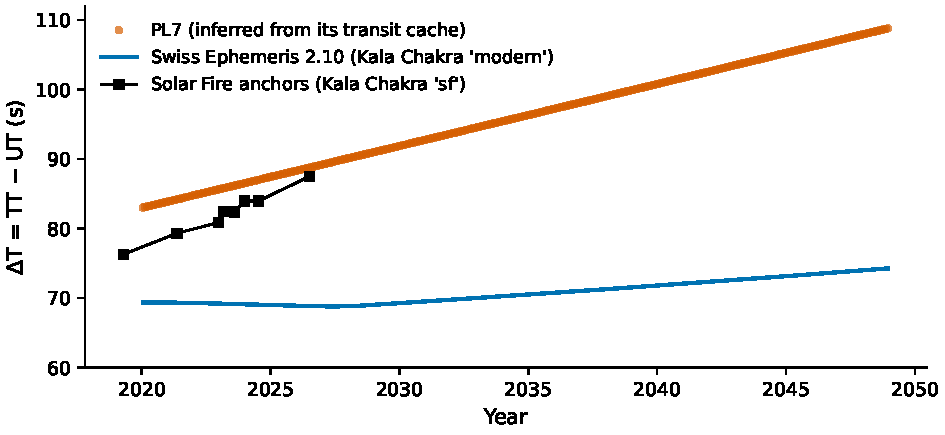
\includegraphics[width=\textwidth]{figures/fig_deltat.pdf}
  \caption[Delta-T used by PL7, Solar Fire and the Swiss Ephemeris]{\textbf{PL7 and Solar
  Fire both over-estimate $\Delta T$; PL7 by 14--20~s over 2020--2026.} \emph{What is
  shown.} Orange points: $\Delta T$ implied by PL7's cached Moon longitudes, one point per
  cached month (348 months, 2020--2048), obtained by dividing the Moon residual against the
  Swiss Ephemeris by the Moon's speed. Blue line: the Swiss Ephemeris~2.10 value used by
  Kala Chakra's \emph{modern} mode. Black squares: the eight Solar Fire anchors used by
  Kala Chakra's \emph{sf} mode (\texttt{ephemeris.js}). \emph{What to take from it.} In the
  years the family uses (2020--2026) PL7's $\Delta T$ is 1--5~s larger than Solar Fire's,
  which moves the Moon by about 1--3$''$; planets are unaffected at the arcsecond level.}
  \label{fig:deltat}
\end{figure}

\ksimple $\Delta T$ only matters for the Moon. A 5-second disagreement moves the Moon by
about $3''$, which is far below the width of a KP sub (the smallest is $40'$), so
this difference is harmless for star and sub lords.

\subsection{Ayanamsa}
\label{sec:ayanamsa}

The ayanamsa is computed in a single routine, \texttt{fcn.0055d3ea}, that is short enough
to decode completely \tagBIN. It first evaluates a Lahiri polynomial,
\begin{equation}
  A_{\text{Lahiri}} = 22^\circ 27' 37.65'' + 5026.87434''\,T + 1.11113''\,T^2,
  \qquad T = \frac{\mathrm{JD} - 2451545}{36525} + 1,
  \label{eq:lahiri}
\end{equation}
where $T$ is Julian centuries from the epoch J1900.0 (JD~2415020.0). A one-byte setting
(offset \texttt{0x67e} of the options object) then selects one of eight branches. For
branches~3--8 a second time argument is used,
\begin{equation}
  t' = \frac{\mathrm{JD} - 2415020.5}{36524},
  \label{eq:tprime}
\end{equation}
which is centuries of 36\,524 days counted from 1900~January~0.5. The widget-to-selector
mapping was recovered from the dialog constructor (\texttt{0x4c01b0}, which names each
radio button and stores it at a fixed member offset) and the OK handler
(\texttt{0x4c6ef0}, which writes the selector according to the checked button)
\tagBIN. The result is \autoref{tab:ayanamsa}. Finally the routine returns
$C - A$, where $C$ is the value typed in the ``offset'' box of the dialog
(\texttt{calculations\_offsetEdit}, default~0); sidereal longitude is tropical longitude
plus this return value.

\begin{table}[htbp]
  \centering
  \small
  \caption[PL7's eight ayanamsa options]{PL7's ayanamsa options as decoded from
  \texttt{fcn.0055d3ea}. ``Value 2025'' is at 2025~January~1 0h~UT. ``vs SE'' is PL7
  minus the Swiss Ephemeris ayanamsa of the same name (mean equinox, 2025); ``vs KC'' is
  PL7 minus Kala Chakra's effective ayanamsa (Swiss Lahiri $- 1.251''$).}
  \label{tab:ayanamsa}
  \begin{tabularx}{\textwidth}{c l >{\raggedright\arraybackslash}X r r r}
    \toprule
    Sel. & Button & Formula ($A$ in degrees) & Value 2025 & vs SE & vs KC \\
    \midrule
    1 & Lahiri (default) & \autoref{eq:lahiri} & 24°12$'$23.0$''$ & $+0.2''$ & $+1.4''$ \\
    2 & None & $0$ (tropical / sayana) & 0 & -- & -- \\
    3 & Yukteshwar & $21.015 + 1.5\,t'$ \;(54$''$/yr) & 22°53$'$24.2$''$ & $+223''$ & -- \\
    4 & Raman & $21.013888889 + 1.398148148\,t'$ & 22°45$'$41.8$''$ & $+5.7''$ & -- \\
    5 & Bhasin & $21.363888889 + 1.398148148\,t'$ & 23°06$'$41.8$''$ & n/a & -- \\
    6 & Fagan--Bradley & $23.348888889 + 1.398148148\,t'$ & 25°05$'$47.8$''$ & $+25''$ & -- \\
    7 & Krishnamurti & $22.453973785 + 1.3955235417\,t'$ & 24°11$'$54.3$''$ & $+320''$ & $-27''$ \\
    8 & Krishnamurti New & $A_{\text{Lahiri}} - 0.101388 + 0.0011118\,t'$ & 24°06$'$23.0$''$ & $-11''$ & $-359''$ \\
    \bottomrule
  \end{tabularx}
\end{table}

Three results matter for the family's work \tagNUM:

\begin{enumerate}[leftmargin=*]
  \item \textbf{PL7's Lahiri is the same Lahiri as Kala Chakra's.} Over 1900--2050 it
  agrees with the Swiss Ephemeris \texttt{SIDM\_LAHIRI} to within $0.3''$, and with Kala
  Chakra's Solar-Fire-calibrated value to $1.4''$. Lahiri charts from the two programs
  therefore agree on every star and sub lord except for points lying within $1.4''$ of a
  boundary (0.02\,\% of random longitudes).
  \item \textbf{``Krishnamurti'' (selector~7) is the classical 291~AD straight-line
  formula.} $22.453974^\circ$ at 1900 with $50.2388''$~yr$^{-1}$ is exactly zero
  ayanamsa in 291~AD at Krishnamurti's published rate of $50.2388475''$~yr$^{-1}$
  ($1609 \times 50.2388'' = 22.454^\circ$). Today it is only $27''$ smaller than Lahiri,
  and it differs from the Swiss Ephemeris's \texttt{SIDM\_KRISHNAMURTI} by about $5'20''$.
  \item \textbf{``Krishnamurti New'' (selector~8) is Lahiri minus $6'05''$} (plus a drift
  of $4''$ per century). It is within $11''$ of the Swiss Ephemeris KP ayanamsa. If a PL7
  user selects it, about 6.8\,\% of all longitudes acquire a different star or sub lord
  from the Lahiri value Kala Chakra uses (\autoref{sec:compare}).
\end{enumerate}

\begin{keybox}\kidea The family's charts are cast in Lahiri. PL7 at its default setting uses
the same Lahiri ayanamsa as Kala Chakra to within $1.4''$. The two KP options in PL7 are
genuinely different ayanamsas, and Kala Chakra offers neither.\end{keybox}

\subsection{True or mean equinox (nutation)}

With the Swiss Ephemeris's nutation switched off (\texttt{SEFLG\_NONUT}), PL7's cached
Rahu agrees with the Swiss true node minus \autoref{eq:lahiri} to $-0.54'' \pm 0.02''$ in
January~2020, and to within $\pm 0.8''$ in every month to 2048; with nutation switched on
the residual is $-16.6''$, which is exactly the nutation in longitude $\Delta\psi$ at
that date \tagNUM. PL7 therefore measures sidereal longitudes from the \emph{mean}
equinox of date. This is the same convention that the Swiss Ephemeris applies internally
in sidereal mode, so it is \emph{not} a difference from Kala Chakra.

\subsection{Rahu and Ketu: true node}

The cached Rahu matches the Swiss Ephemeris \emph{true} node to sub-arcsecond precision
and differs from the mean node by up to $1.4^\circ$ in a month \tagNUM. PL7 uses the true
node, as does Kala Chakra. Ketu is diametrically opposite.

\subsection{House cusps: Placidus, always}
\label{sec:placidus}

The chart-calculation method (code at \texttt{0x55fefc}) calls one cusp routine,
\texttt{fcn.00406c94}, unconditionally: there is no branch on any house-system setting
before the call \tagBIN. That routine carries the debug labels \texttt{plac cusp 0}
\ldots\ \texttt{plac cusp 4}. It computes the ascendant and MC, then for the intermediate
cusps calls an iterative helper (\texttt{fcn.0040684a}) with the fractions 1/3 and 2/3 and
the angular offsets $30^\circ$, $60^\circ$, $120^\circ$, $150^\circ$, using
\texttt{atan}: the textbook semi-arc trisection that defines the Placidus system
\tagBIN. The twelve cusps are written to an array at offset \texttt{0xf0}; elements~0 and~9
(cusp~1 and cusp~10) are then copied to the ascendant and MC fields. The dialog has no
house-system option; the manual's discussion of bhavas is in \autoref{sec:bhava}.

\begin{keybox}\kidea Your father was right: PL7 casts Placidus cusps. Kala Chakra casts
Topocentric (Polich--Page) cusps, which is what Solar Fire Gold was set to.\end{keybox}

\paragraph{Latitude.} The executable contains no WGS84 constant (neither
$(1-f)^2 = 0.99330562$ nor $1 - e^2$), so PL7 almost certainly feeds the \emph{geographic}
latitude to the house formula, whereas Kala Chakra converts it to \emph{geocentric}
latitude, reproducing Solar Fire's ``geocentric correction to latitude'' option \tagINF.

\paragraph{How large is the difference?} Using the Swiss Ephemeris house functions for
2000 random moments in 2019--2026, \autoref{tab:cusps} compares PL7's method (Placidus,
geographic latitude) with Kala Chakra's (Topocentric, geocentric latitude) at the two
canonical places \tagNUM. Placidus and Topocentric cusps on their own differ by only a few
arcseconds at these latitudes; almost all of the difference comes from the latitude
convention, which shifts the ascendant--descendant axis.

\begin{table}[htbp]
  \centering
  \small
  \caption[Placidus (PL7) versus Topocentric (Kala Chakra) cusps]{Absolute difference
  between PL7-style cusps (Placidus, geographic latitude) and Kala Chakra cusps
  (Topocentric, geocentric latitude), in arcseconds, over 2000 random moments in
  2019--2026. Cusps 4 and 10 coincide by construction. ``Flip'' is the share of all cusps
  whose star or sub lord differs.}
  \label{tab:cusps}
  \begin{tabular}{l rrrrrr r}
    \toprule
     & \multicolumn{6}{c}{Cusp (mean / max, $''$)} & \\
    \cmidrule(lr){2-7}
    Place & 1 \& 7 & 2 \& 8 & 3 \& 9 & 4 \& 10 & 5 \& 11 & 6 \& 12 & Flip \\
    \midrule
    Singapore ($1.28^\circ$N) & 8 / 12 & 6 / 8 & 3 / 4 & 0 / 0 & 3 / 4 & 5 / 8 & 0.1\,\% \\
    Lapanga ($21.70^\circ$N) & 149 / 227 & 126 / 209 & 71 / 122 & 0 / 0 & 70 / 122 & 125 / 209 & 1.7\,\% \\
    \bottomrule
  \end{tabular}
\end{table}

\subsection{Yogi point}
\label{sec:yogi}

\texttt{fcn.0040841f} returns $\mathrm{norm}_{360}(\lambda_\odot + \lambda_\text{Moon} +
93^\circ 20')$, using sidereal longitudes \tagBIN; the constant $93.3333\ldots$ is stored at
\texttt{0x5d1948}. This is the standard Yogi point. Its callers also compute nakshatra
indices with the helper \texttt{fcn.00566b15} (nakshatra $= 1 + \lfloor \lambda / 13^\circ
20' \rfloor$) and wrap them into $1\ldots27$; the documented definitions of Avayogi and
the Duplicate Yogi are given in \autoref{sec:yogidoc}.
